La web application dispone di una homepage che riporta i dati più significativi inerenti alla stazione.

\begin{figure}[H]
    \begin{center}
    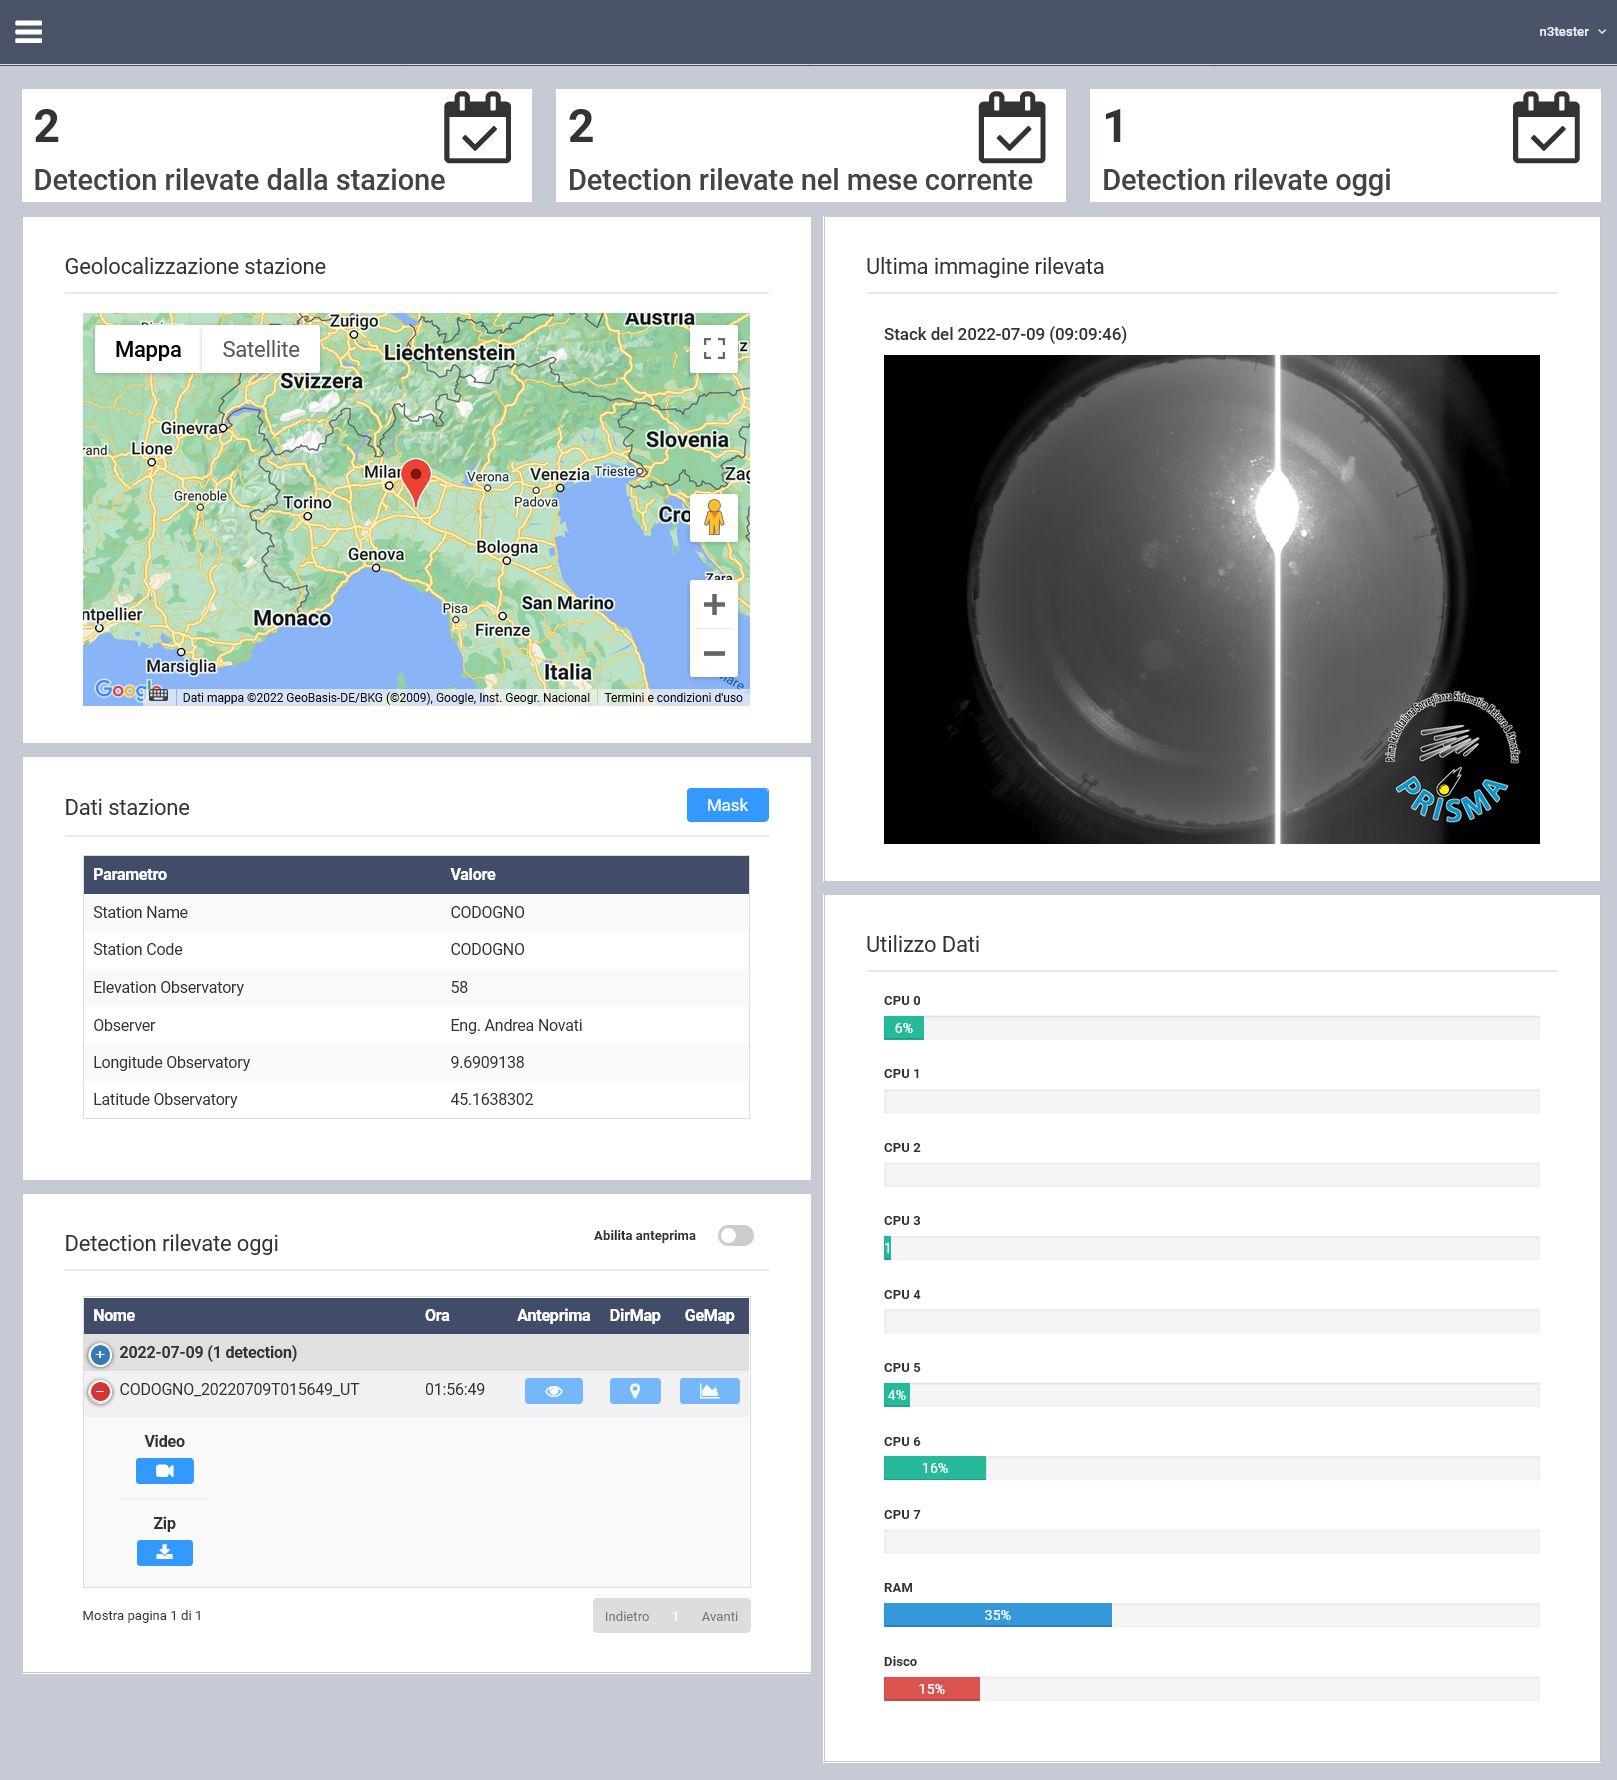
\includegraphics[width=\textwidth]{images/full-home.png}
    \caption{\emph{Homepage} della web application.}
    \label{fig:homepage}
    \end{center}
\end{figure}

\subsection{Visualizzazione metriche}

All'inizio della pagina sono indicati alcuni dati numerici relativi alle detection rilevate:
\begin{itemize}[noitemsep,nolistsep]
    \item Numero di detection rilevate dalla stazione \textbf{totali}
    \item Numero di detection rilevate dalla stazione \textbf{nel mese corrente}
    \item Numero di detection rilevate dalla stazione \textbf{oggi}
\end{itemize}

\begin{figure}[H]
    \begin{center}
    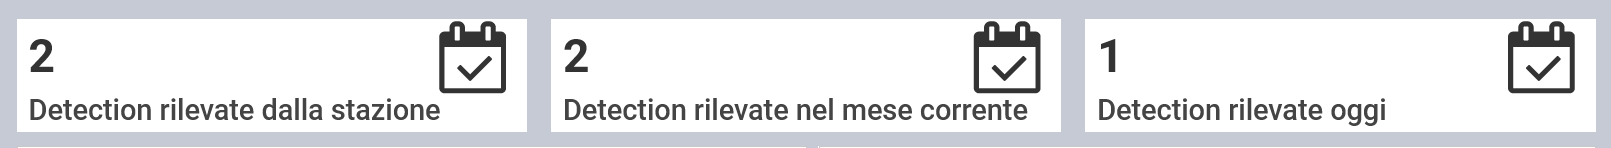
\includegraphics[width=\textwidth]{images/metriche.png}
    \caption{Metriche.}
    \end{center}
\end{figure}

\subsection{Geolocalizzazione e informazioni della stazione}

L'utente può visualizzare le \textbf{informazioni principali} della stazione (cfr. sezione \ref{ft-conf-automatica}) in una tabella; la \textbf{geolocalizzazione}, realizzata con GoogleMaps, (cfr. figura \ref{fig:homepage}) ed infine, se presente, la \textbf{maschera}, mostrata in una finestra modale, con possibilità di download.

\begin{figure}[H]
    \begin{center}
    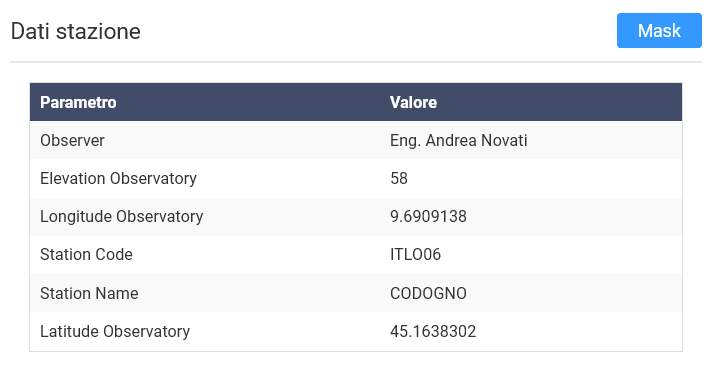
\includegraphics[width=\textwidth]{images/dati-stazione.png}
    \caption{Dati princiapli della stazione.}
    \end{center}
\end{figure}
\begin{figure}[H]
    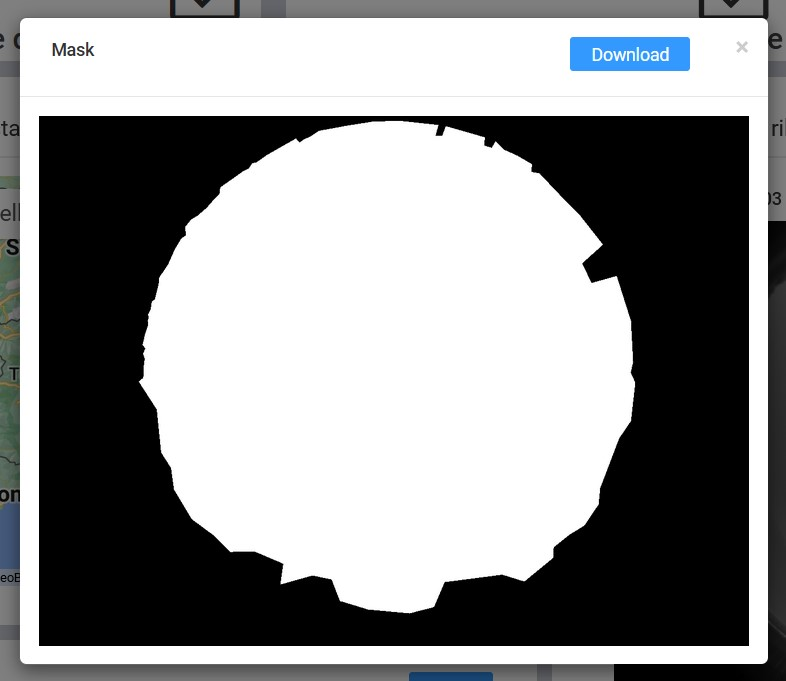
\includegraphics[width=\textwidth]{images/mask.jpg}
    \caption{Anteprima della maschera.}
\end{figure}

\subsection{Visualizzazione ultime detection}

Sotto i dati della stazione, si possono consultare le detection rilevate nell'ultimo giorno. La tabella in questione coincide con la seconda tabella nella sezione \emph{Detection}, associata all'ultima data disponibile (cfr. sezione \ref{detec-tables}).

Viene inoltre riportata nella homepage l'immagine dell'\textbf{ultimo stack}, che coincide con l'ultima immagine rilevata dalla stazione.

\subsection{Visualizzazione stato risorse dell'hardware} \label{stato-risorse-hw}

L'utente visionando la homepage può avere una panoramica dell'\textbf{utilizzo delle risorse} sul nodo (cfr. figura \ref{fig:homepage}). Sono infatti riportati:
\begin{itemize}[noitemsep,nolistsep]
    \item Utilizzo \textbf{CPU} (è riportato l'utilizzo di ciascun core)
    \item Utilizzo \textbf{RAM}
    \item Occupazione \textbf{disco}
\end{itemize}

Il client effettua una richiesta al server ogni 5 secondi per aggiornare i dati. 

Il server per trovare l'utilizzo di ciascun core tramite il software sysstat (cfr. sezione \ref{software}) esegue il comando \texttt{mpstat}, ricavando i dati necessari con \texttt{awk} (cfr. listing \ref{lst:system-usage}).

\begin{lstlisting}[style=PHP,caption={Metodo PHP per ottenere l'utilizzo di CPU, RAM e disco.},captionpos=b,label={lst:system-usage}]
    // Get percentage values of cpu, ram and disk usage
    public static function getStoragePercentage() {
        $disk = ((disk_total_space("/") 
            - disk_free_space("/"))
            / disk_total_space("/")) * 100;
        $cpu = array();
        $i = 0;
        while (true) {
            $core = shell_exec("mpstat -P $i 1 1 | awk
                'FNR==4
                {print($3+$4+$5+$6+$7+$8+$9+$10+$11)}'");
            if (is_null($core)) {
                break;
            }
            $cpu[] = (float) str_replace("\n", "", $core);
            $i++;
        }
        $free1 = shell_exec('free');
        $free2 = (string) trim($free1);
        $free_arr = explode("\n", $free2);
        $mem1 = explode(" ", $free_arr[1]);
        $mem2 = array_filter($mem1);
        $mem3 = array_merge($mem2);
        $ram = $mem3[2] / $mem3[1] * 100;
        return array($cpu, $ram, $disk);
    }
\end{lstlisting}